% Fig. 2 -- Pipeline overview (vector, standalone).
% Compile:  pdflatex fig2_pipeline.tex   ->  fig2_pipeline.pdf
% Design rule: every module is either LEARNED (blue, solid) or a GEOMETRIC
% RULE (grey, dashed). The paper states explicitly that only endpoint linking
% is learned inside the graph stage; pruning is a deterministic size rule.
\documentclass[border=2pt]{standalone}
\usepackage[T1]{fontenc}
\usepackage{helvet}
\renewcommand{\familydefault}{\sfdefault}
\usepackage{tikz}
\usetikzlibrary{arrows.meta,positioning,calc}

\definecolor{learnc}{RGB}{32,102,172}
\definecolor{geoc}{RGB}{105,105,112}
\definecolor{learnfill}{RGB}{232,241,250}
\definecolor{geofill}{RGB}{240,240,242}

\begin{document}
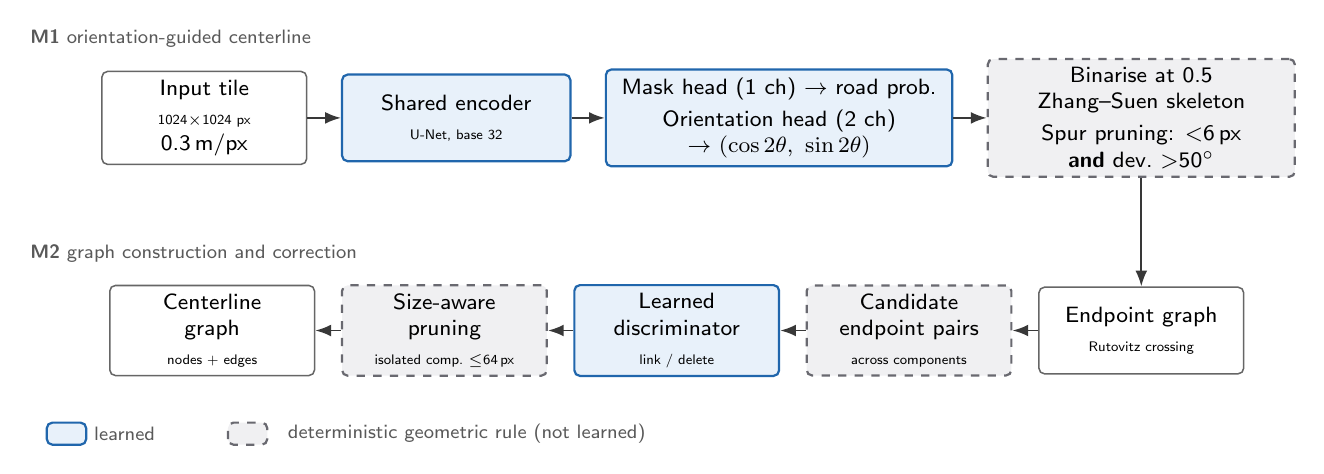
\begin{tikzpicture}[
    font=\footnotesize,
    >={Latex[length=2.0mm,width=1.5mm]},
    box/.style={draw, rounded corners=2pt, align=center, inner sep=3pt,
                minimum height=1.10cm, line width=0.55pt},
    learned/.style={box, draw=learnc, fill=learnfill, line width=0.8pt},
    geo/.style={box, draw=geoc, fill=geofill, dashed, line width=0.8pt},
    data/.style={box, draw=black!60, fill=white},
    arr/.style={->, line width=0.7pt, draw=black!78},
    lbl/.style={font=\scriptsize, text=black!65, inner sep=1pt},
    tiny/.style={font=\scriptsize},
  ]

  % ================= Row 1 (left to right): mask + orientation branch
  \node[data, minimum width=2.6cm] (in) at (1.70,3.60)
       {Input tile\\[1pt]\tiny 1024$\times$1024 px\\0.3\,m/px};
  \node[learned, minimum width=2.9cm] (enc) at (4.90,3.60)
       {Shared encoder\\[1pt]\tiny U-Net, base 32};
  \node[learned, minimum width=4.4cm] (heads) at (9.00,3.60)
       {Mask head (1 ch) $\rightarrow$ road prob.\\[2pt]
        Orientation head (2 ch)\\[0pt]
        $\rightarrow$ $(\cos 2\theta,\ \sin 2\theta)$};
  \node[geo, minimum width=3.9cm] (skel) at (13.60,3.60)
       {Binarise at 0.5\\[0pt]
        Zhang--Suen skeleton\\[2pt]
        Spur pruning: $<$6\,px\\[0pt]
        \textbf{and} dev.\ $>$50$^\circ$};

  % ================= Row 2 (right to left): graph stage
  \node[data, minimum width=2.6cm] (graph) at (13.60,0.90)
       {Endpoint graph\\[1pt]\tiny Rutovitz crossing};
  \node[geo, minimum width=2.6cm] (cand) at (10.65,0.90)
       {Candidate\\endpoint pairs\\[1pt]\tiny across components};
  \node[learned, minimum width=2.6cm] (link) at (7.70,0.90)
       {Learned\\discriminator\\[1pt]\tiny link / delete};
  \node[geo, minimum width=2.6cm] (prune) at (4.75,0.90)
       {Size-aware\\pruning\\[1pt]\tiny isolated comp.\ $\leq$64\,px};
  \node[data, minimum width=2.6cm] (out) at (1.80,0.90)
       {Centerline\\graph\\[1pt]\tiny nodes + edges};

  % ================= arrows
  \draw[arr] (in) -- (enc);
  \draw[arr] (enc) -- (heads);
  \draw[arr] (heads) -- (skel);
  \draw[arr] (skel) -- (graph);
  \draw[arr] (graph) -- (cand);
  \draw[arr] (cand) -- (link);
  \draw[arr] (link) -- (prune);
  \draw[arr] (prune) -- (out);

  % ================= stage labels
  \node[lbl, anchor=south west] at (-0.55,4.45)
       {\textbf{M1} orientation-guided centerline};
  \node[lbl, anchor=south west] at (-0.55,1.72)
       {\textbf{M2} graph construction and correction};

  % ================= legend
  \begin{scope}[shift={(-0.30,-0.55)}]
    \filldraw[draw=learnc, fill=learnfill, rounded corners=2pt, line width=0.8pt]
      (0,0) rectangle (0.50,0.28);
    \node[lbl, anchor=west] at (0.56,0.14) {learned};
    \filldraw[draw=geoc, fill=geofill, dashed, rounded corners=2pt, line width=0.8pt]
      (2.30,0) rectangle (2.80,0.28);
    \node[lbl, anchor=west] at (3.02,0.14)
      {deterministic geometric rule (not learned)};
  \end{scope}

\end{tikzpicture}
\end{document}
